\section{Non-uniform Robustness: Decidability at order four}
\label{section:decidability2}
\begin{figure}[h]

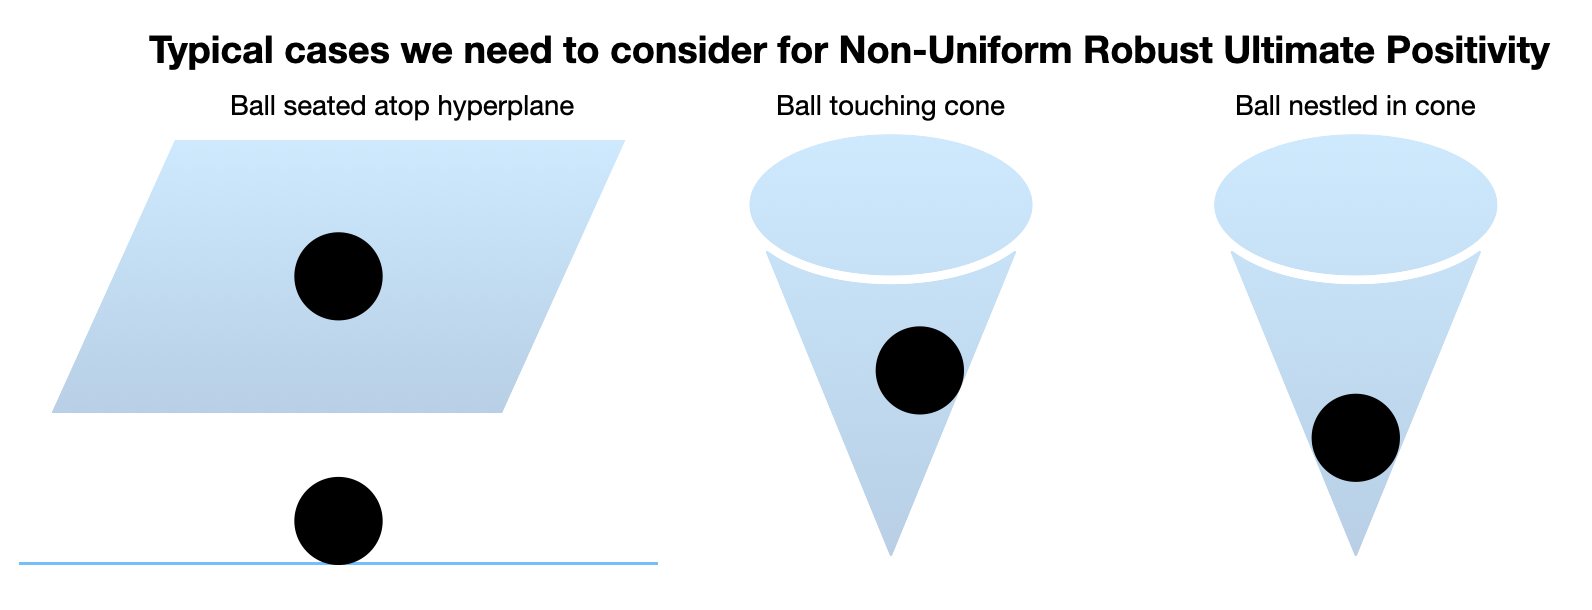
\includegraphics[width=\textwidth]{picture1.png}
\caption{Visual intuition}
\label{fig:geometricpicture}
\end{figure}

In this section, we prove Theorem \ref{thm:decide2}. As before, the techniques naturally apply to lower orders, and we omit their explicit treatment. Recall equation \ref{eq:grouping} and the surrounding discussion:
\begin{equation}
u_n/n^d\rho^n = \begin{bmatrix}
{\color{red!70!black} \mathbf{q}_{dom}^T(n) } & \mathbf{q}_{res}^T(n)
\end{bmatrix}
\begin{bmatrix}
{\color{red!70!black} \mathbf{p}_{dom}} \\
\mathbf{p}_{res}
\end{bmatrix}
\end{equation}
The crucial first task is to check whether for all points $\mathbf{p'}$ in the neighbourhood, \\$\liminf_{n\in\naturals}\seq{\mathbf{q}_{dom}(n), \mathbf{p'}_{dom}} = \mu(\mathbf{p'}) \ge 0$. Although Ultimate Positivity is guaranteed for the points where the inequality is strict, the neighbourhood may intersect the critical region where $\mu = 0$. If there are no non-dominant terms, this is irrelevant; but otherwise decidability hinges on whether we can handle the intersection.

Recall Proposition \ref{prop:folklore}: for Ultimate Positivity, there \textit{must} be a real positive dominant root. We make cases, based on the presence of a pair of complex conjugates among the dominant roots. If the dominant terms are all real, then there are at most two of them, and $\seq{\mathbf{q}_{dom}(n), \mathbf{p'}_{dom}} \ge 0$ is the intersection of at most two halfspaces (of the form $z - |w| \ge 0$). The neighbourhood must lie entirely above the separating hyperplanes (ball atop hyperplane in Figure \ref{fig:geometricpicture}). The points where the neighbourhood is tangent to the planes have algebraic coordinates. The polynomial equations for the coordinates come from the facts that: (i) the point lies on the plane, (ii) the point lies on the surface of the neighbourhood, (iii) the gradient of $(\mathbf{p'} - \mathbf{p})^T\mathbf{M}(\mathbf{p'} - \mathbf{p})$ is along the normal to the plane. Alternately, one could simply use the First Order Theory of the Reals, as discussed below. Solving for critical points of tangency gives us low-order, decidable instances of Ultimate Positivity.

Otherwise, the dominant terms contain a pair of complex conjugates. The case where the remaining root is $-1$ (dominant) is similar, and simpler. We thus assume $\seq{\mathbf{q}_{dom}(n), \mathbf{p'}_{dom}} = z + x\cos n\theta + y\sin n\theta$. We assume $\theta$ is not a rational multiple of $2\pi$ (can be detected, Theorem \ref{thm:abelian}): otherwise, the region where $\mu(\mathbf{p'}) \ge 0$ is again a finite union of halfspaces, which can be handled as before. Recall equation \ref{eq:liminfmin}. We get that $\mu(\mathbf{p'}) = z -\sqrt{x^2 + y^2}$. As shown in Figure \ref{fig:geometricpicture}, the critical region $\mu(\mathbf{p'}) = 0$ is a cone. Consider the following first order formula, which conveys that the dominant contribution for all points in the neighbourhood is guaranteed to be non-negative.
\begin{equation}
\label{eq:firsttask}
\chi_0 := \forall \mathbf{p'}.~ (\mathbf{p'} - \mathbf{p})^T\mathbf{M}(\mathbf{p'} - \mathbf{p}) \le 1 \Rightarrow \mu(\mathbf{p'}) \ge 0
\end{equation}
We can use Theorem \ref{thm:renegar} (Renegar) to evaluate the truth of this sentence in the First Order Theory of the Reals. If $-1$ is a root, we adjust the expression for $\mu$ accordingly. Here, evaluating the truth of the formula suffices to decide Ultimate Positivity, because there are no non-dominant terms.

Thus, we concentrate on the case where there is one non-dominant term, i.e. $\seq{\mathbf{q_n}, \mathbf{p'}} = z + x\cos n\theta + y\sin n\theta + w\alpha^n$. As discussed, we need to analyse the points where the (surface of the) neighbourhood intersects the region $\mu(\mathbf{p'}) = 0$, and where the non-dominant terms can make a negative contribution. Notice that the cone $z - \sqrt{x^2 + y^2} = 0$ is carved out by \textit{infinitely} many hyperplanes of the form $z + x\cos\phi + y\sin\phi = 0$. Consider the following first order formula with free variable $c$
\begin{equation}
\label{eq:intersection}
\chi_1(c):= \exists s \exists \mathbf{p'}.~ (\mathbf{p'} - \mathbf{p})^T\mathbf{M}(\mathbf{p'} - \mathbf{p}) = 1 \land z + cx + sy = 0 \land c^2 + s^2 = 1 \land w \sim 0
\end{equation}

In the above $\sim$ is $\ne$ if the non-dominant root $\alpha < 0$, and is $<$ otherwise. ($\alpha$ is necessarily nonzero!) The free variable $c$ stands for $\cos \phi$, and denotes the hyperplane where the neighbourhood, which lies within the cone, possibly touches the surface of the cone. Moreover, by the inequalities on $w$, we also enforce that the non-dominant terms make a negative contribution at the point of contact. We can use Theorem \ref{thm:renegar} to get an equivalent quantifier free formula: this comprises purely of polynomial (in-)equalities in the free variable $c$. The set of $c$, and hence $\cos \phi$, satisfying these, consists of finitely many intervals. Of course, Ultimate Positivity is guaranteed when this set is empty: the non-dominant terms are never adversarial when the dominant contribution is dangerously small.

We first dispose of the case where all intervals consist of single points. Consider an interval $\{c_0\}$ consisting of a single point. This is illustrated by the case of the ball touching the cone in Figure \ref{fig:geometricpicture}. Since we know that for the corresponding witness $s_0, z_0, x_0, y_0$, $z_0 \ge \sqrt{x_0^2 + y_0^2}$, it must be the case that $x_0 = -z_0c_0$, $y_0 = -z_0s_0$. Since $c_0, s_0$ are algebraic; regardless of $z_0, w_0$, this point of tangency is an order 4 decidable instance of Ultimate Positivity: in fact, it is a YES instance, due to the techniques of \cite{ouaknine2014ultimate}.

If, however, the set of $c$ satisfying $\chi_1$ consists of intervals that have more than one point, then the techniques of \cite{ouaknine2014ultimate} to decide Ultimate Positivity for a single point with algebraic coordinates are no longer accessible. This situation is illustrated by the case of the ball nestled in cone in Figure \ref{fig:geometricpicture}. Let $[\phi_1, \phi_2]$ be an interval of $\phi$ such that: a) all values of $c$ between $\cos\phi_1$ and $\cos\phi_2$ satisfy $\chi_1$, b) The corresponding witnesses $z$ are at most $z_0$, and c) The corresponding witnesses $w$ have magnitude at least some fixed $w_0$. Then, we must have for each $\phi$ (and corresponding $z(c), x = -cz, y = -z\sin \phi, w)$) in this interval, the following inequality is violated only finitely often:
\begin{equation}
z - z\cos(n\theta - \phi) + w\alpha^n \ge 0
\end{equation}

We consider an even weaker inequality, which, in this context, we argue is bound to be violated infinitely often:
\begin{equation}
z_0[n\theta - \phi]_{2\pi}^2  \ge 2w_0\alpha^n
\end{equation}

The argument hinges on Lemma \ref{lemma:existsreal}, which we restate:
\begin{lemma}
\label{lemma:existsreal3}
For every irrational number $x$, strictly decreasing real positive function $\psi$, and interval $\mathcal{I} = [a, b] \subset [0, 1], ~ a \ne b$, there exists $y \in \mathcal{I}$ such that $[nx - y] < \psi(n)$ for infinitely many odd, and infinitely many even $n$.
\end{lemma}

Now, if $\alpha < 0$, we use Lemma \ref{lemma:existsreal3} on the irrational $\theta/2\pi$, an irrational, and the decreasing $\sqrt{\frac{w_0 |\alpha|^n}{2\pi^2z_0}}$ to argue that there exists a $\phi$ in the desired interval, such that the weaker inequality will be violated for infinitely many $n$ of the the appropriate parity. Thus, we can return NO if we are in the case where the set of $c$ satisfying $\chi_1$ (equation \ref{eq:intersection}) consists of intervals that contain more than a single point.

